\documentclass[10pt,twocolumn]{extarticle}

\usepackage[margin=0.58in,columnsep=0.24in]{geometry}
\usepackage[T1]{fontenc}
\usepackage{lmodern}
\usepackage{microtype}
\usepackage{booktabs}
\usepackage{tabularx}
\usepackage{array}
\usepackage{graphicx}
\usepackage{xcolor}
\usepackage{enumitem}
\usepackage[font=footnotesize,labelfont=bf]{caption}
\usepackage{titlesec}
\usepackage{hyperref}
\usepackage{flushend}

\hypersetup{colorlinks=true,linkcolor=blue!40!black,citecolor=blue!40!black,
  urlcolor=blue!50!black,
  pdftitle={Controlled Testing and Failure Attribution for ML Sensor Pipelines},
  pdfauthor={Working proposal}}
\setlength{\parindent}{0pt}
\setlength{\parskip}{1.2pt}
\setlist{nosep,leftmargin=*,topsep=1pt}
\titlespacing*{\section}{0pt}{3pt}{1pt}
\titleformat{\section}{\small\bfseries}{\thesection}{0.4em}{}
\newcolumntype{Y}{>{\raggedright\arraybackslash}X}

\title{\vspace{-1.55em}\textbf{Controlled Testing and Failure Attribution\\[-0.18em]
for ML Sensor Pipelines}\\[-0.15em]
\normalsize Two-page Paper 3 proposal}
\author{Working proposal for postdoc and advisor review}
\date{27 July 2026}

\begin{document}
\maketitle
\vspace{-1.9em}

\begin{abstract}
Post-training monitors can flag distribution change but rarely distinguish a
sensor/acquisition shift from unsupported physical states or a broken
evaluation contract. We propose a controlled, replay-based study of that
distinction---not a maintained software product. Declared interventions,
named representation hooks, deterministic contract gates, and calibrated
abstention are evaluated across NuBench point clouds and a fixed waveform
reconstruction task. Against input tests, MMD, classifier two-sample tests,
embedding distance, uncertainty, and output-only monitoring, we measure
detection power and delay, false alerts, failure-family attribution, latency,
storage, and reproducibility. The intended result is quantitative: generic
monitors detect N/S shifts, layerwise evidence improves attribution, and
deterministic gates isolate evaluation faults at measured replay cost.
\end{abstract}

\section{Scope, continuity, and novelty}

Paper~1 identifies likelihood geometry under structured noise; Paper~2
separates residual geometry, architecture class, and training support. Paper~3
asks whether those contracts can be tested after training. Its artifact is a
reproducible experiment suite---configurations, adapters, hooks, replay
scripts, and reports---not a branded platform or a promise of production
maintenance.

The contribution is a controlled cross-modal design that combines (i) paired
sensor perturbations, support-composition shifts, and deliberate contract
faults; (ii) feature-matched attribution comparisons with guarded abstention;
and (iii) a power--cost study of full capture, sampling, reservoirs, and
fixed-dimensional sketches. NuBench, the waveform-noise generator, and MMD are
inputs to that design, not claimed inventions. Cross-geometry results test
consistency, not causal detector-design effects.

\section{Failure contracts and claims}

We predeclare three labels. \textbf{N---acquisition/noise shift} includes PSD
or covariance change, jitter, drift, spectral lines, glitches, tails, hit
thinning, and channel/module loss. \textbf{S---training-support shift} changes
window composition toward physical strata that are sparse under the clean
training distribution; events themselves are not corrupted. \textbf{E---evaluation-
contract fault} includes wrong units, coordinate ordering, output semantics,
PSD convention, or metric implementation. E is not a distribution shift and
is not the likelihood-metric mismatch studied in Papers~1--2.

\textbf{C1---Detect N/S shifts.} At a 1\% false-alert rate on nominal,
non-overlapping windows, the best monitoring signature detects at least 80\%
of held-out abrupt and gradual N/S shifts within five windows and is
non-inferior to the strongest eligible baseline by a five-point power margin.
Delay is primary in events and simulated seconds.

\textbf{C2---Attribute with abstention.} A fixed classifier over statistical
monitors plus deterministic gates reaches macro-F1 $\geq0.80$ on held-out
N/S/E cases. For N/S, the full layerwise signature exceeds the same classifier
using all generic-monitor outputs by $\geq0.20$ F1. Split-conformal distance in
standardized fingerprint space must identify an unseen family with AUROC
$\geq0.80$ instead of forcing a known label. This is intervention-family
attribution, not unrestricted physical root-cause discovery.

\textbf{C3---Trade power for cost.} Ten-percent event sampling plus fixed-size
sketches yields p95 replay-path latency overhead $<10\%$, at least $10\times$
less representation storage, and no more than five points of power/F1 loss
relative to full capture. Effects and intervals are repeated across modalities,
three NuBench model families, two machines, and CPU/GPU where supported. These
targets are frozen after development profiling and power analysis.

\begin{figure*}[t]
  \centering
  \begin{minipage}[b]{0.43\textwidth}
    \centering
    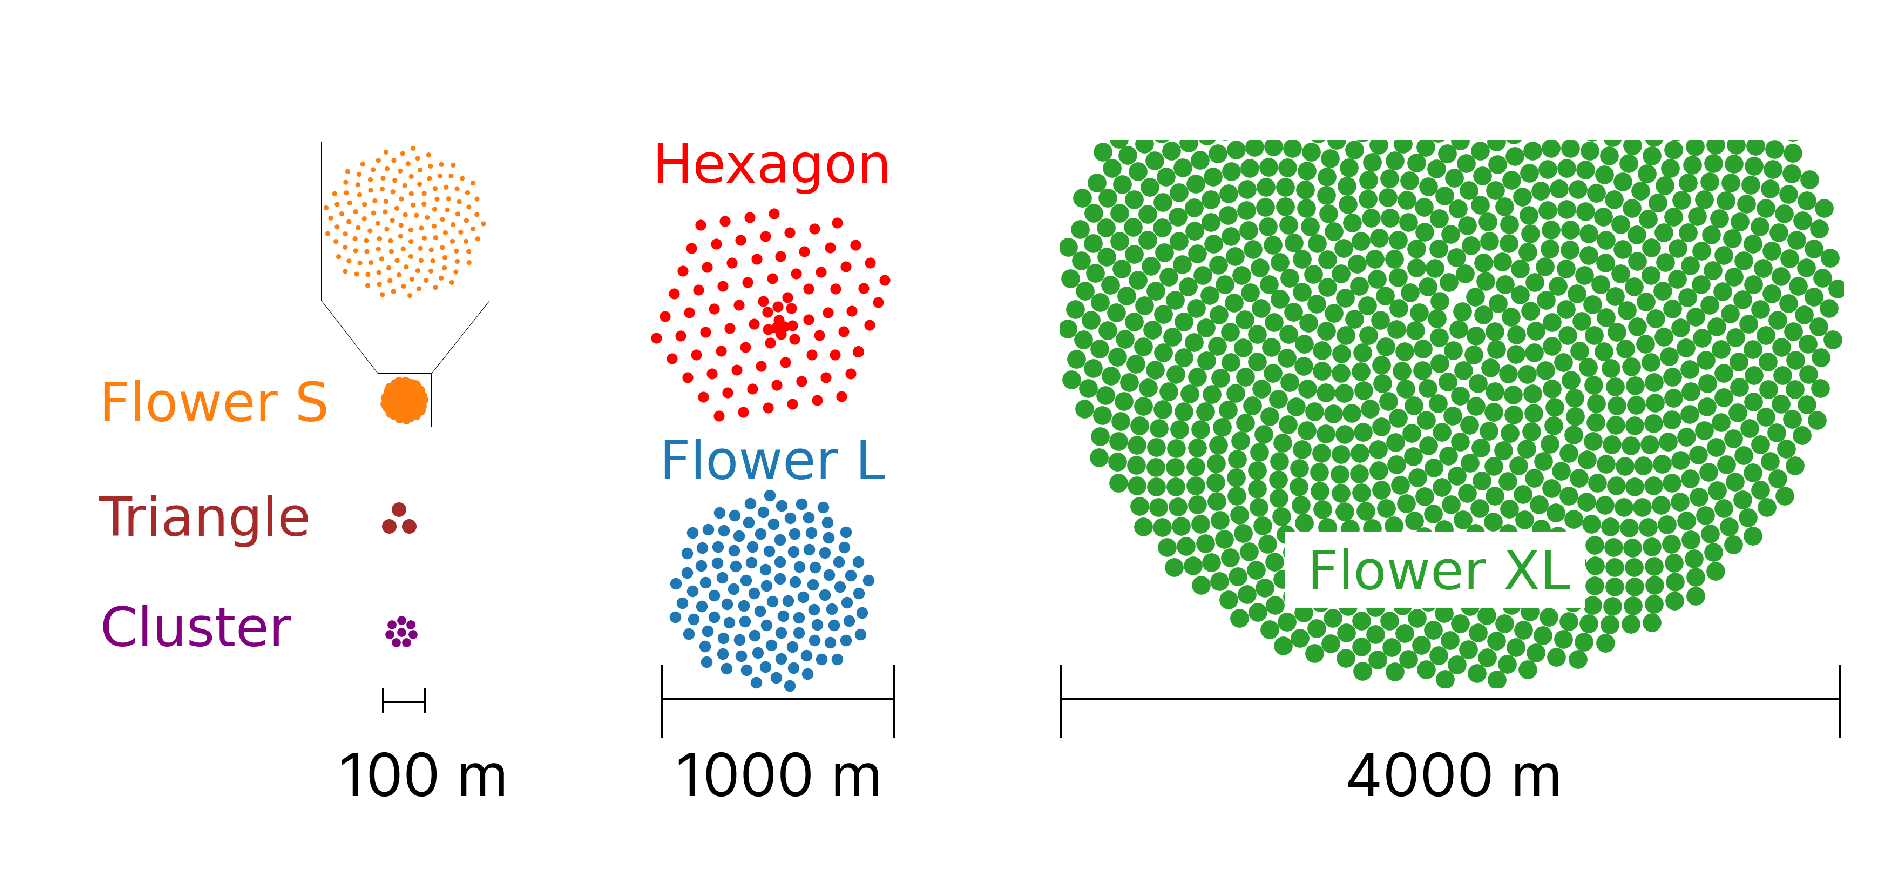
\includegraphics[width=\linewidth,height=1.50in,keepaspectratio]{figures/nubench_detector_geometries.png}\\[-0.2em]
    \scriptsize (a) NuBench detector geometries
  \end{minipage}\hfill
  \begin{minipage}[b]{0.25\textwidth}
    \centering
    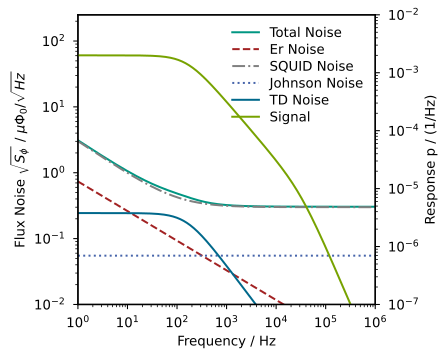
\includegraphics[width=\linewidth,height=1.50in,keepaspectratio]{figures/spectrum_detector_signal_noise.png}\\[-0.2em]
    \scriptsize (b) detector signal/noise spectrum
  \end{minipage}\hfill
  \begin{minipage}[b]{0.28\textwidth}
    \centering
    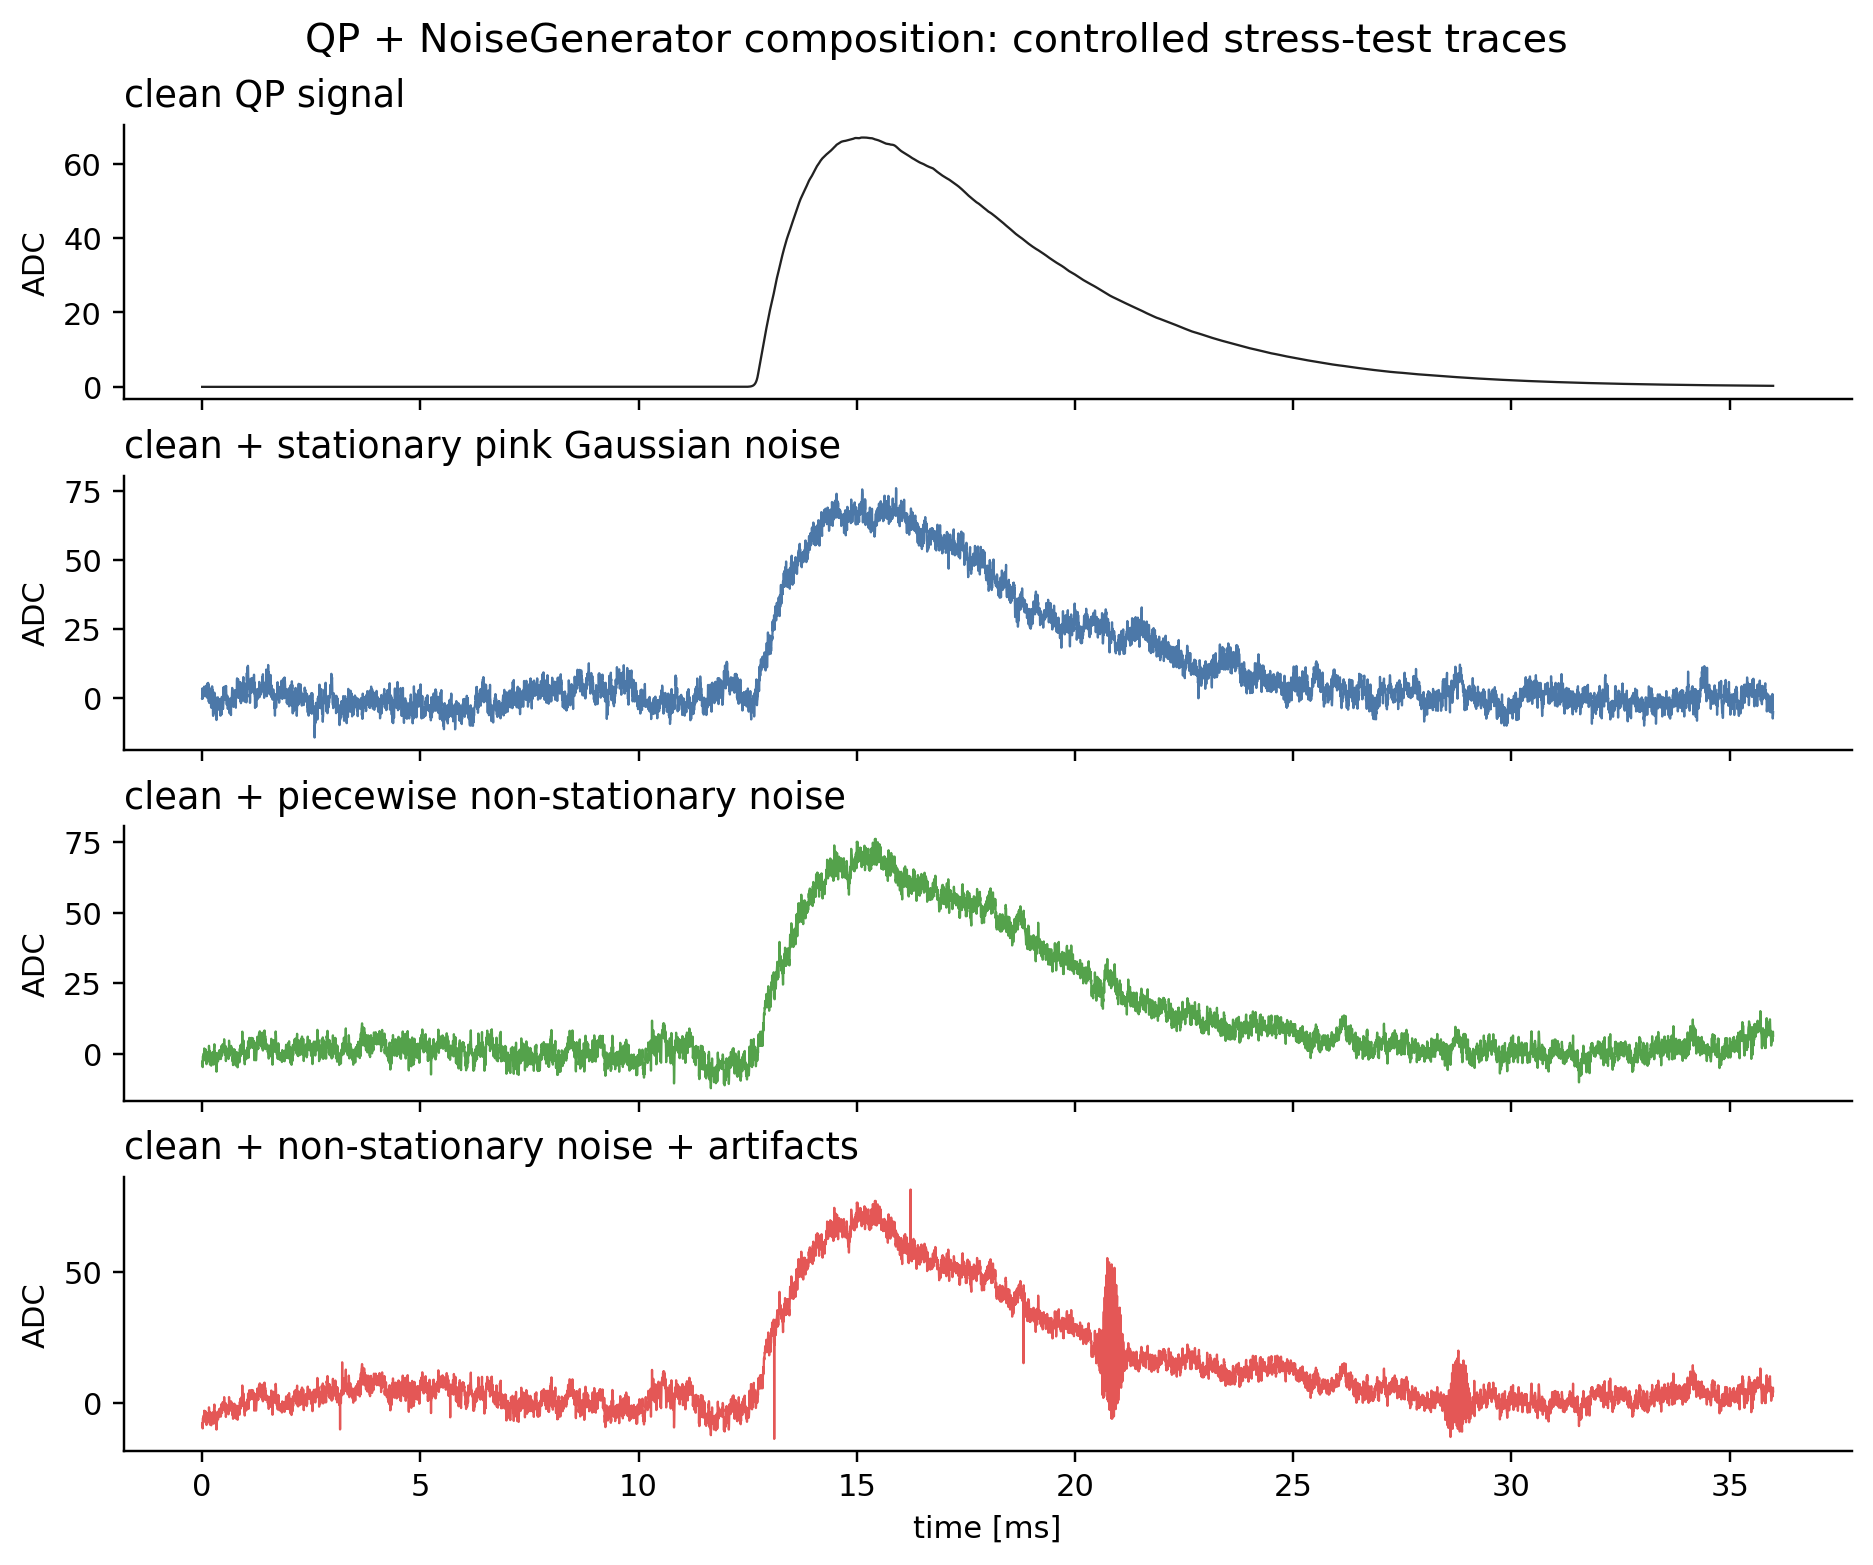
\includegraphics[width=\linewidth,height=1.50in,keepaspectratio]{figures/noise_generator_examples.png}\\[-0.2em]
    \scriptsize (c) generated waveform stress tests
  \end{minipage}
  \vspace{-0.45em}
  \caption{Complementary testbeds. (a) Six top-view geometries, reproduced
  from NuBench Fig.~3~\cite{nubench}. (b) The supplied Al$_2$O$_3$/Al
  athermal-detector response and component PSDs. (c) The generator composes a
  clean optimal-filter-like pulse with stationary colored noise, piecewise
  nonstationarity, and explicit artifacts. Panels (b)--(c) are project outputs.}
  \label{fig:testbeds}
  \vspace{-0.7em}
\end{figure*}

\section{Methods and testbeds}

Each event window records input-quality summaries, named-layer moments or
sketches, outputs, uncertainty, delayed task metrics, and calibration. Eligible
N/S baselines receive identical windows and false-alert budgets: corrected
univariate input tests, RBF-MMD~\cite{gretton2012}, a classifier two-sample
test~\cite{lopezpaz2017}, final-embedding mean/covariance distance, output
tests, and uncertainty/entropy. A regularized logistic classifier is fitted
with identical splits to five arms: input only; output/uncertainty; final
embedding only; all generic-monitor outputs; and the full layerwise signature.
E uses schema/range invariants and clean-reference tests, not drift statistics.
Clean miscalibration is a model result, not automatically a software bug
\cite{guo2017}; latent displacement is normalized by clean within-class
dispersion.

\textbf{NuBench point clouds.} The first cell is Hexagon Ice LE $\times$
DynEdge $\times$ direction. The restored 1,358,099-parameter checkpoint exposes
a 128-D pre-head event representation. Module dropout, hit thinning, and time
jitter instantiate N. S windows use clean low-density strata in energy,
topology, vertex/containment, and multiplicity, estimated from training only.
ParticleNeT and GRIT repeat the study; another geometry is a consistency check
\cite{nubench}.

\textbf{Waveforms and the noise module.} The fixed task uses non-overlapping
4096-sample windows at 10~MS/s, a rank-2 noise-aware EMPCA encoder fitted on the
chronological training split, and sinusoid-amplitude reconstruction. The module
accepts or constructs PSD/CSD models, samples seeded frequency-domain random
coefficients with the required real-signal symmetry, transforms them into time
traces, and adds stationary color, piecewise nonstationarity, lines, drift,
glitches, and tails to clean signals (Fig.~\ref{fig:testbeds}b--c). It validates
units and second-order spectral statistics. It is therefore a controlled N
intervention engine, not another dataset, reconstruction model, or physical-
source separator. S holds out declared frequency/amplitude ranges; E swaps
coefficient order or frequency units and changes PSD/score conventions.

\begin{center}
\centering
\scriptsize
\captionof{table}{Confirmatory experiment matrix. Drift baselines apply only to N/S.}
\begin{tabularx}{\columnwidth}{@{}p{0.18in}p{1.05in}Y@{}}
\toprule
ID & Test & Primary endpoints \\
\midrule
E0 & Clean replay; deliberate E faults & Reference discrepancy; gate sensitivity/specificity \\
E1 & Held-out abrupt/gradual N/S & Power at 1\% false alert; AUROC/AUPRC; delay \\
E2 & N/S/E, mixtures, unseen family & Macro/multi-label F1; confusion; unknown AUROC \\
E3 & Capture vs sample/reservoir/sketch & p50/p95 latency; bytes/event; power/F1 loss \\
E4 & Models, modalities, hardware & Scaling; interval agreement; report hashes \\
\bottomrule
\end{tabularx}
\label{tab:experiments}
\vspace{-0.6em}
\end{center}

Held-out severities, seeds, support strata, N+S mixtures, and one unseen family
prevent perturbation lookup. Windows and thresholds are frozen after
development. Intervals resample event groups and perturbation seeds separately.
Cost sweeps event rate, window size, hook count, embedding dimension, and model
count; repeat runs record machine, accelerator, timing method, and data/config
hashes. Null results require a passed positive control, adequate precision, and
a predeclared equivalence margin.

\section{Smoke test and feasibility gate}

The selected 8.82~GiB NuBench release is checksummed; the DynEdge checkpoint
restores and the 128-D hook runs. Rescoring all 2,989,339 released predictions
reproduces published median angular errors within $0.055^\circ$:
$23.6548^\circ$ versus $23.60^\circ$ for CC/track and $56.1553^\circ$ versus
$56.12^\circ$ for NC/cascade. This misses a deliberately strict $0.01^\circ$
identity tolerance. On 256 development events, checkpoint and released
directions differ by $0.944^\circ$ median ($7.708^\circ$ p95); therefore the
clean gate remains open. A module-dropout positive control is monotone
($15.28^\circ\!\to25.12^\circ$ median angular error; 10-NN retention
$1.000\!\to0.393$ from 0--50\% dropout), establishing perturbation, hook, and
paired-metric feasibility without presenting the pilot as a scientific claim.

\begin{thebibliography}{5}
\scriptsize
\setlength{\itemsep}{-0.5pt}
\bibitem{nubench} R.~F. \O rs\o e et al. ``NuBench: An Open Benchmark for Deep
Learning-Based Event Reconstruction in Neutrino Telescopes.'' JINST 21 (2026).
\href{https://arxiv.org/abs/2511.13111}{arXiv:2511.13111}.
\bibitem{gretton2012} A. Gretton et al. ``A Kernel Two-Sample Test.'' JMLR 13
(2012), 723--773.
\bibitem{lopezpaz2017} D. Lopez-Paz and M. Oquab. ``Revisiting Classifier
Two-Sample Tests.'' ICLR (2017).
\bibitem{guo2017} C. Guo et al. ``On Calibration of Modern Neural Networks.''
ICML (2017).
\end{thebibliography}

\end{document}
